\renewcommand{\this}{BayesianNetworks}

\chapter{Bayesian Networks}
This chapter is partially based on 
\textit{A Tutorial on Learning With Bayesian Networks} and Christopher
M. Bishops classic \textit{Pattern Recognition and Machine Learning}.
\\\\
In this chapter, we will go over the basics of 
Bayesian networks. In essence, Bayesian networks
are a compact representation over a set of
random variables. They are a subset of the so called
Probabilistic Graphical Models (PGM) which are more
commonly referred to as graphical models. Graphical
models express conditional independence between 
variables using graphs, hence their name.
Bayesian networks have become somewhat popular and
used in quite a few applications. Many libraries
provide easy development using Bayesian networks.
\\\\
This section is structured as follows. First we delve
deeper into \textit{directed acyclic graphs} (DAGs), which
is used to encode conditional independence in Bayesian
networks. We look into the definition of Bayesian,
which turn out to be quite simple yet elegant. A
big downside to Bayesian networks, however, is the
computational complexity. Thirdly, we have a look 
at exact inference in Bayesian networks. Then we
look at approximate inference.

\section{Conditional independence as a DAG}
Graphical models are based on graphs to encode conditional independence 
in probability distributions. In the case of Bayesian networks conditional
independence is encoded as a \textit{directed acyclic graph}, or more 
commonly referred to as DAGs. DAGs are defined as follows:

\begin{defn}[Directed Acyclic Graph]
A graph $G = (V, E)$ is called acyclic when the edges $E$ are directed
and the graph contains no directed cycles. A directed cycle is a 
sequence of connected edges such that at least one vertex is visited 
twice.
\begin{equation}
\lnot \exists x_1, x_2 \dots x_n \in V: (x_i, x_{i+1}) \in E \text{ and }
	x_1 = x_n
\end{equation}
\end{defn}

\noindent
As an example figure \ref{fig:example_DAG} shows two graphs 
over the vertex set $V=\{A, B, C, D\}$. The left graph is a DAG
as there is no vertex from which there is a sequence of directed
edges which result in the same vertex. The right graph does 
contain a directed cycle. For example the path defined by $ACDA$.

\begin{figure}[h!]
\centering

\begin{minipage}[c]{0.3\textwidth}
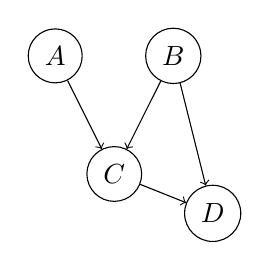
\begin{tikzpicture}
	\draw (0,0) node[shape=circle, draw=black](a){$A$};
	\draw (1.5,0) node[shape=circle, draw=black](b){$B$};
	\draw (0.75,-1.5) node[shape=circle, draw=black](c){$C$};
	\draw (2,-2) node[shape=circle, draw=black](d){$D$};
	
	\draw [->](a) -- (c);
	\draw [->](b) -- (c);
	\draw [->](b) -- (d);
	\draw [->](c) -- (d);
\end{tikzpicture}
\end{minipage}
\begin{minipage}[c]{0.3\textwidth}
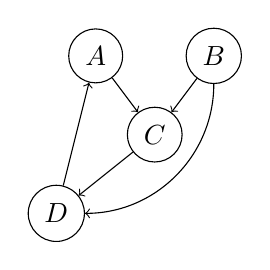
\begin{tikzpicture}

	\draw (0,0) node[shape=circle, draw=black](a){$A$};
	\draw (1.5,0) node[shape=circle, draw=black](b){$B$};
	\draw (0.75,-1.0) node[shape=circle, draw=black](c){$C$};
	\draw (-0.5,-2) node[shape=circle, draw=black](d){$D$};
	
	\draw [->](a) -- (c);
	\draw [->](b) -- (c);
	\draw [->](b.south) to [out=270, in= 0] (d.east);
	\draw [->](c) -- (d);
	\draw [->](d) -- (a);
\end{tikzpicture}
\end{minipage}
\caption{Example of a DAG (left) and a graph with a directed
cycle (right).}
\label{fig:example_DAG}
\end{figure}

\noindent
A crucial and simple concept in DAGs is the concept of parents.
\begin{defn}[Parents in a DAG]
Given a vertex $v \in V$ in a DAG $G=(V, E)$ the parents of 
$v$ are all the vertices for which an outgoing edge ends in $v$:
\begin{equation}
Pa(v) = \{ u \in V \mid (u, v) \in E\}
\end{equation}
\end{defn}

\section{Bayesian networks with DAGs}
What do these DAGs have to do with Bayesian networks? As mentioned
earlier in the context of Bayesian networks they define conditional
independence between variables. Let us first define Bayesian networks:

\begin{defn}[Bayesian networks]
A Bayesian network over variables $\textbf{X}=\{X_1,\dots X_k\}$
is a graph-probability pair $(G, \Theta)$. The graph $G$ is a DAG
which encodes conditional independence. The vertices $V$ in $G$ are
in a one-to-one correspondence with the variables $\textbf{X}$. We
do not make a distinction between the random variable $X_i \in 
\textbf{X}$ and the graph node $X_i \in V$. In this definition 
$\Theta$ is a collection of local conditional probabilities for 
each variable $X_i \in \textbf{X}$. The set $\Theta$ is defined as:
\begin{equation}
\Theta = \{P(X_i | Pa(X_i)) | X_i \in \textbf{X}\}
\end{equation}
Together, $G$ and $\Theta$ define a joint probability distribution
over the variables $\textbf{X}$:
\begin{equation}
p(\textbf{X} = x) = \prod_{i=1}^{k} p(X_i = x_i | Pa(X_i) = x)
\end{equation}
\end{defn}

\begin{exmp}
This example was taken from Christopher M. Bishop's classic book
\textit{pattern recognition and machine learning}. Let's assume
we are tasked with fitting a polynomial regression to a data set 
$\textbf{x} = \{x_1, \dots, x_n\}$ where $x_i \in \Real^m$ and 
observations $\textbf{y}=\{y_1, \dots, y_n\}$ and wish to predict 
a given new point $x_{n+1}$.
In the case of Bayesian learning, the model parameters $\textbf{W}$
and observations $\textbf{Y}$ will be considered as random variables.
Hence, we also assume a prior over $\textbf{W}$. This prior has one
hyper parameter $\alpha$ and is written as $p(\textbf{W} \mid \alpha)$.
Additionally, the noise parameter $\sigma^2$ and $\alpha$ are
considered known and fixed. The joint distribution over $\textbf{W}$ 
and $\textbf{Y}$ is then:

\begin{equation}
\begin{split}
p(\textbf{W}, \textbf{Y} \mid \textbf{x}, \alpha, \sigma^2) 
	&= p(\textbf{W} \mid \alpha, \sigma^2, \textbf{x})
	   \prod_{i=1}^{n} p(Y_i \mid \textbf{W}, \alpha, \sigma^2, \textbf{x})\\
	&= p(\textbf{W} \mid \alpha)
	   \prod_{i=1}^{n} p(Y_i \mid \textbf{W}, \sigma^2, x_i)\\
\end{split}
\end{equation}

\noindent
Note that we sometime leave out the fixed parameters to avoid
cluttering the equations too much.
\begin{equation}
\begin{split}
p(\textbf{W}, \textbf{Y} \mid \textbf{x}, \alpha, \sigma^2) 
	&= p(\textbf{W}, \textbf{Y})\\
	&= p(\textbf{W})
	   \prod_{i=1}^{n} p(Y_i \mid \textbf{W})\\
\end{split}
\end{equation}

\noindent
If we map this to a Bayesian network, we obtain the network
depicted in figure \ref{fig:exmpl_BN_poly_regr}. Note the left
figure is the same network, where the blue rectangle is shorthand
notation. Everything in the blue box is duplicated $N$ times.
A vertex being filled with blue indicates that we observed this
random variable. Note that $\alpha$, $\sigma^2$ and $x_i$ 
are not considered random variables, yet for better understanding
they are still depicted.

\begin{figure}[h!]
\centering

\begin{tabular}{cc}
\begin{minipage}[c]{0.55\textwidth}
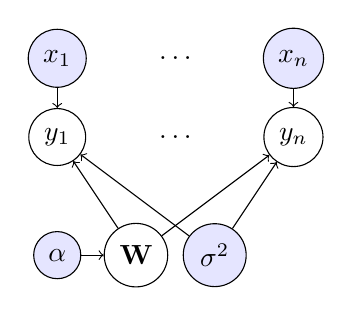
\begin{tikzpicture}
	\draw (0,0) node[shape=circle, 
					 draw=black,
					 fill=blue,
					 fill opacity = 0.1,
					 text opacity = 1.0](x1){$x_1$};
	\draw node[below of = x1, 
			   shape=circle, 
			   draw=black](y1){$y_1$};
	
	\draw (1.5, 0) node[](txt){$\dots$};
	\draw node[below of=txt](txt){$\dots$};
	
	\draw (3,0) node[shape=circle, 
					 draw=black,
					 fill = blue,
					 fill opacity = 0.1,
					 text opacity = 1.0](xn){$x_n$};
	\draw node[below of = xn, 
			   shape=circle, 
			   draw=black](yn){$y_n$};
	
	\draw [->](x1) -- (y1);
	\draw [->](xn) -- (yn);
	
	\draw (0, -2.5) node[shape=circle, 
					 draw=black,
					 fill=blue,
					 fill opacity = 0.1,
					 text opacity = 1.0](alpha){$\alpha$};
	\draw (1, -2.5) node[draw=black, shape=circle](w){$\textbf{W}$};
	\draw (2, -2.5) node[shape=circle, 
					 	draw=black,
					 	fill=blue,
					 	fill opacity = 0.1,
					 	text opacity = 1.0](sigma){$\sigma^2$};
	
	\draw [->](w) -- (y1);
	\draw [->](w) -- (yn);
	\draw [->](sigma) -- (y1);
	\draw [->](sigma) -- (yn);
	\draw [->](alpha) -- (w);
\end{tikzpicture}
\end{minipage}
&
\begin{minipage}[c]{0.4\textwidth}
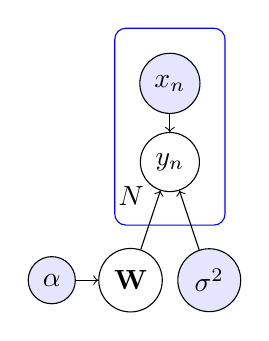
\begin{tikzpicture}
	\draw (1.5,0) node[shape=circle, 
					 draw=black,
					 fill=blue,
					 fill opacity = 0.1,
					 text opacity = 1.0](x1){$x_n$};
	\draw node[below of = x1, 
			   shape=circle, 
			   draw=black](y1){$y_n$};

	\draw [->](x1) -- (y1);
	\draw [draw=blue, rounded corners] (0.8, -1.8) rectangle
		 node[pos = 0.15]{$N$} ++(1.4, 2.5);
		
	\draw (0, -2.5) node[shape=circle, 
					 draw=black,
					 fill=blue,
					 fill opacity = 0.1,
					 text opacity = 1.0](alpha){$\alpha$};
	\draw (1, -2.5) node[draw=black, shape=circle](w){$\textbf{W}$};
	\draw (2, -2.5) node[shape=circle, 
					 	draw=black,
					 	fill=blue,
					 	fill opacity = 0.1,
					 	text opacity = 1.0](sigma){$\sigma^2$};
	
	\draw [->](w) -- (y1);
	\draw [->](sigma) -- (y1);
	\draw [->](alpha) -- (w);
\end{tikzpicture}
\end{minipage}
\end{tabular}
\caption{Bayesian networks for Bayesian polynomial regression.
Left is long, expanded network. Right uses shorthand notation.}
\label{fig:exmpl_BN_poly_regr}
\end{figure}

\noindent
From the network we could then marginalize towards $\textbf{W}$ or
towards $Y_i$:
\begin{equation}
p(\textbf{W} \mid \textbf{Y}) 
= \frac{p(\textbf{W})\prod_{i=1}^{m}p(Y_i \mid \textbf{W})}{p(\textbf{Y})}
\end{equation}
\begin{equation}
p(Y_i \mid \textbf{W}, \textbf{Y}^i) 
= \frac{p(\textbf{W} \mid \alpha)\prod_{i=1}^{m}
	p(Y_i \mid \textbf{W})}{p(\textbf{W}, \textbf{Y}^i)}
\end{equation}

\noindent
This network is not particularly interesting as we already have
the observations $\textbf{y}={y_1, \dots, y_n}$. In order to 
predict a new data point $x_{n+1}$ we can expand our model as follows:
\begin{equation}
p(Y_{n+1}, \textbf{W}, \textbf{Y}\mid x_{n+1})
	= p(\textbf{W})p(Y_{i+1}\mid \textbf{W}, x_{n+1})
	\prod_{i = 1}^{n}p(Y_i\mid \textbf{W})
\end{equation}

\noindent
The Bayesian network corresponding with this model would be an
extension of the model in figure \ref{fig:exmpl_BN_poly_regr}.

\begin{figure}[h!]
\centering

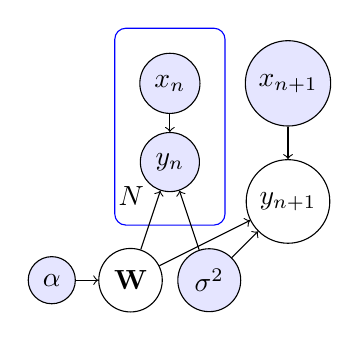
\begin{tikzpicture}
	\draw (1.5,0) node[shape=circle, 
					 draw=black,
					 fill=blue,
					 fill opacity = 0.1,
					 text opacity = 1.0](x1){$x_n$};
	\draw node[below of = x1, 
			   shape=circle, 
			   draw=black,
			   fill = blue,
			   fill opacity = 0.1,
			   text opacity = 1.0](y1){$y_n$};
			   
	\draw (3,0) node[shape=circle, 
					 draw=black,
					 fill=blue,
					 fill opacity = 0.1,
					 text opacity = 1.0](xn1){$x_{n+1}$};
	\draw (3, -1.5)node[shape=circle, 
			   draw=black](yn1){$y_{n+1}$};

	\draw [->](x1) -- (y1);
	\draw [->](xn1) -- (yn1);
	
	\draw [draw=blue, rounded corners] (0.8, -1.8) rectangle
		 node[pos = 0.15]{$N$} ++(1.4, 2.5);
		
	\draw (0, -2.5) node[shape=circle, 
					 draw=black,
					 fill=blue,
					 fill opacity = 0.1,
					 text opacity = 1.0](alpha){$\alpha$};
	\draw (1, -2.5) node[draw=black, shape=circle](w){$\textbf{W}$};
	\draw (2, -2.5) node[shape=circle, 
					 	draw=black,
					 	fill=blue,
					 	fill opacity = 0.1,
					 	text opacity = 1.0](sigma){$\sigma^2$};
	
	\draw [->](w) -- (y1);
	\draw [->](sigma) -- (y1);
	\draw [->](alpha) -- (w);
	\draw [->](sigma) -- (yn1);
	\draw [->](w) -- (yn1);
\end{tikzpicture}
\end{figure}

\noindent
To make this example more clear. We could for example assume several
conditional probability distributions. Take for example 
$p(Y_i \mid \textbf{W})$, in the case of polynomial regression
it could for instance signify:
\begin{equation}
p(Y_i \mid \textbf{W}, x_i) = \mathcal{N}\big(f(\textbf{W}, x_i), V\big)
\end{equation}
The prior over $\textbf{W}$ could be chosen as a Gaussian with
zero mean and some diagonal variance matrix:
\begin{equation}
p(\textbf{W} \mid \alpha) = \mathcal{N}\big( \textbf{0}, \alpha \ID\big)
\end{equation}
\end{exmp}

\section{Discrete variables in Bayesian networks}
We've seen Bayesian networks as defining a joint probability
over a set of random variables $\textbf{X}$. We can apply
the Bayesian network principle to a set of discrete variables.
In fact, Bayesian networks are usually introduced as a way to
compactly define a distribution over discrete variables.
The rest of this chapter, we will consider the random variables
of a Bayesian network as discrete. However, keep in mind that 
this doesn't have to be the case.

\subsection{Full joint probabilities}
When dealing with discrete variables, one usually uses multinomial 
distributions. Given a discrete variable $X$, which can take on
$K$ values from $1$ to $K$ with probabilities 
$\mu = \{\mu_1, \dots, \mu_K\}$. The probability 
distribution of $X$ is given by:
\begin{equation}
p(X \mid \mu) = \prod_{i=1}^{K} {\mu_i}^{x_i}
\end{equation}
Where $x_i$ indicates whether $X$ has taken value $i$. To define
this distribution, one would need exactly $K - 1$ parameters. We
subtract $1$ as the condition $\sum \mu_i = 1$ must hold and we
lose a degree of freedom. For a single variable this is not yet a
problem. However, what happens when we have a join distribution over
$m$ variables, where each variable can assume $K$ values?
In this case the probability distribution would look as follows:
\begin{equation}
p(X_1, \dots, X_m) = p(X_1)p(X_2 \mid X1)\dots p(X_m \mid X_1, \dots, X_{m-1})
\end{equation}
For each $p(X_i \mid X_1, \dots, X_{i-1})$ we need exactly $K^{i-1}(K - 1)$
parameters to define it. We derive it mathematically:
\begin{equation}
\sum_{i=1}^{m} K^{i-1}(K - 1) = K^m -1
\end{equation}
The proof for this equation can be found in the definitions
section at the start.
In total we obtain exactly $K^m - 1$ parameters
needed to fully define the joint distribution. This is of course
unmanageable in any real world context. There are several ways 
one could combat this. One way is by imposing an independence structure
in the form of Bayesian networks. Take for example a joint probability
distribution over $\textbf{X} = \{A, B, C, D\}$, each taking values in
$\{1, 10\}$. This network would consist of $10^{4} - 1 = 9999$ 
parameters. If we use for example the network in figure
\ref{fig:BN_exmaple_params}, we would only use $9 + 90 + 900 + 90 
= 1089$ 
parameters.
\begin{figure}[h!]
\centering
\begin{minipage}[c]{0.3\textwidth}
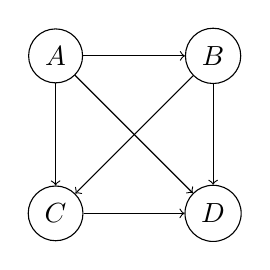
\begin{tikzpicture}
	\draw (0, 0) node[draw = black,
					  shape = circle
			   ](A){$A$};
	\draw (2, 0) node[draw = black,
					  shape = circle
			   ](B){$B$};
	\draw (0, -2) node[draw = black,
					  shape = circle
			   ](C){$C$};
	\draw (2, -2) node[draw = black,
					  shape = circle
			   ](D){$D$};
			   
	\draw[->] (A) -- (B);
	\draw[->] (A) -- (C);
	\draw[->] (A) -- (D);
	
	\draw[->] (B) -- (C);
	\draw[->] (B) -- (D);
	
	\draw[->] (C) -- (D);
\end{tikzpicture}
\end{minipage}
\begin{minipage}[c]{0.3\textwidth}
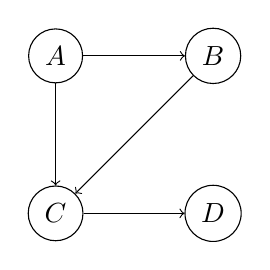
\begin{tikzpicture}
	\draw (0, 0) node[draw = black,
					  shape = circle
			   ](A){$A$};
	\draw (2, 0) node[draw = black,
					  shape = circle
			   ](B){$B$};
	\draw (0, -2) node[draw = black,
					  shape = circle
			   ](C){$C$};
	\draw (2, -2) node[draw = black,
					  shape = circle
			   ](D){$D$};
			   
	\draw[->] (A) -- (B);
	\draw[->] (A) -- (C);
	
	\draw[->] (B) -- (C);
	
	\draw[->] (C) -- (D);
\end{tikzpicture}
\end{minipage}
\caption{Example of fully connected Bayesian network (left) and
not fully connected Bayesian network (right).}
\label{fig:BN_exmaple_params}
\end{figure}

\noindent
Using Bayesian networks, we can
easily reduce the amount of parameters even further. For example
by parameter sharing between connections, referred to as \textit{tying}
parameters. Take for example the connections $p(B \mid A)$ and 
$p(D \mid C)$. If we assume they share parameters we would instead
have $9 + 900 + 90 = 999$ parameters. Lastly another simple method
of reducing the number of parameters is by using parameterized models
for example a logistic regression. As an example, take variable $C$
in figure \ref{fig:BN_exmaple_params}. We could define $C$ as:
\begin{equation}
p(C \mid A, B) = \sigma\Big( w_0 + w_1 A + w_2 B \Big)
\end{equation}

\section{Conditional independence by BNs}
An important property in Bayesian networks is conditional independence:
\begin{defn}
Two variables $A$ and $B$ are conditionally independent given $C$ 
if and only if:
\begin{equation}
p(A \mid B, C) = p(A \mid C)
\end{equation}
Intuitively, if we have information about $C$ then any information
we have about $B$ is irrelevant for the outcome of $A$. Conditional
independence shall be denoted as $A \CI B \mid C$.
\end{defn}

\noindent
The significance of conditional independence will become clear later
when looking at inference in Bayesian networks. We can represent 
$A \CI B \mid C$ in a Bayesian network as depicted in figure
\ref{fig:BN_CI_ABC}. This is because 
$p(A, B \mid C) = p(A \mid C)p(B \mid C)$.

\begin{figure}[h!]
\centering
\begin{minipage}{0.3\textwidth}
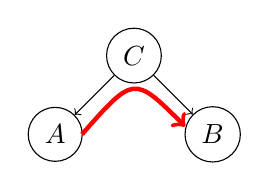
\begin{tikzpicture}
	\draw (0,0) node[draw = black,
					 shape = circle](A) {$A$};
	\draw (1, 1)node[draw = black,
					 shape = circle](C) {$C$};
	\draw (2, 0)node[draw = black,
					 shape = circle](B) {$B$};
					 
	\draw[->] (C) -- (A);
	\draw[->] (C) -- (B);
	
	\draw[red, ->, ultra thick] (0.34,0) .. controls (1, 0.75) .. (1.65,0.1);
\end{tikzpicture}
\end{minipage}
\begin{minipage}{0.3\textwidth}
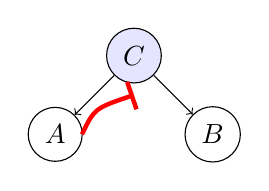
\begin{tikzpicture}
	\draw (0,0) node[draw = black,
					 shape = circle](A) {$A$};
	\draw (1, 1)node[draw = black,
					 shape = circle,
					 fill = blue,
					 fill opacity = 0.1,
					 text opacity = 1.0](C) {$C$};
	\draw (2, 0)node[draw = black,
					 shape = circle](B) {$B$};
					 
	\draw[->] (C) -- (A);
	\draw[->] (C) -- (B);
	
	\draw[red, -|, ultra thick] (0.34,0) .. controls (0.5, 0.33) .. (1,0.5);
	
\end{tikzpicture}
\end{minipage}

\caption{Depiction of $A$ is independent of $B$ given $C$. 
Left, the information can flow from $A$ to $B$, because $C$
is unknown. Right the 
information is blocked, because $C$
is known.}
\label{fig:BN_CI_ABC}
\end{figure}

\noindent
Of course, this conditional independence does not mean $A$ and $B$
are independent variables. If $C$ is not given, information about $A$
may very well influence the outcome of $B$. We notice that information
\textit{travels} from $A$ to $B$ if $C$ is unknown. Conversely, 
information in \textit{blocked} from $A$ to $B$ if $C$ is known.

\section{D-separation}
In this section we have a closer look at the previous observation.
How does information \textit{travel} throughout the Bayesian net
given specific observations? Which variables are conditionally 
independent from each other given a certain set of other variables?
Is there an easy way to verify these by using the DAG?
\\\\
To investigate these questions further, we first look at the 
three building blocks in Bayesian networks. Each of the building
blocks are Bayesian networks with exactly three nodes. For
each of them we will observe how information travels from one
node to another. From there, we can define a notion of conditional
independence between groups of variables in more complex Bayesian
networks.

\subsection{Building block: one}
This 3 node network has already been discussed. Namely the network 
in figure \ref{fig:BN_CI_ABC}. We've already mentioned that $C$
will \textit{block} information flow from $A$ to $B$ if it is given.
\begin{exmp}
Consider $A=$ whether or not you have a runny nose.
$B = $ Whether or not you have a fever. $C=$ whether or not you 
have the flu. Clearly, if you know you have the flu $C = 1$, then
whether or not you have a runny nose $A = 1$ is independent
from whether or not you have a fever $B = 1$. However, if $C$ is
unknown, one might expect to have a higher chance of a runny nose 
($A = 1$) if you already have a fever ($B = 1$).
\end{exmp}

\noindent
We can verify that, in general $A \not \CI B$:
\begin{equation}\begin{split}
p(A, B) 
	&= \sum_c p(A, B \mid c)p(c)\\
	&= \sum_c p(A \mid c)p(B \mid c)p(c)
\end{split}\end{equation}
This is of course not equal to $p(A)(B)$ in the general case. 
However, with information about $C$ we do find independence:
\begin{equation}\begin{split}
p(A, B \mid c) 
	&= \frac{p(c)p(A \mid c)p(B \mid c)}{p(c)} \\
	&= p(A \mid c) p(B \mid c)
\end{split}\end{equation}
We conclude that $A \not \CI B$ and $A \CI B \mid C$.
\subsection{Building block: two}
The second building block is shown in figure \ref{fig:building_block_two}.
In this case we find a very similar situation as building block one.
If $C$ is known, information is \textit{blocked} from $A$ to $B$.
However, information flows freely from $A$ to $B$ if $C$ is unknown.

\begin{figure}[h!]
\centering
\begin{minipage}{0.4\textwidth}
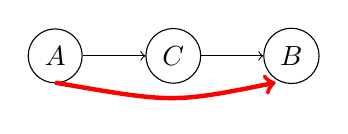
\begin{tikzpicture}

	\draw (0,0) node[draw = black,
					 shape = circle] (A) {$A$};
	
	\draw (3,0) node[draw = black,
					 shape = circle] (B) {$B$};
					 
	\draw (1.5,0) node[draw = black,
					 shape = circle] (C) {$C$};
					 
	\draw[->] (A) -- (C);
	\draw[->] (C) -- (B);
	
	\draw[red, ultra thick, ->] (0, -0.34) .. 
			controls (1.5, -0.6) .. (2.8, -0.34);
\end{tikzpicture}
\end{minipage}
\begin{minipage}{0.4\textwidth}
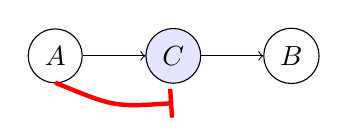
\begin{tikzpicture}

	\draw (0,0) node[draw = black,
					 shape = circle] (A) {$A$};
	
	\draw (3,0) node[draw = black,
					 shape = circle] (B) {$B$};
					 
	\draw (1.5,0) node[draw = black,
					 shape = circle,
					 fill = blue,
					 fill opacity = 0.1,
					 text opacity = 1.0] (C) {$C$};
					 
	\draw[->] (A) -- (C);
	\draw[->] (C) -- (B);
	
	\draw[red, ultra thick, -|] (0, -0.34) .. 
			controls (0.75, -.65) .. (1.5, -0.6);
\end{tikzpicture}
\end{minipage}
\caption{The second building block for D-separation. 
Left, the information can flow from $A$ to $B$, because $C$
is unknown. Right the 
information is blocked, because $C$
is known.}
\label{fig:building_block_two}
\end{figure}
\begin{exmp}
Consider $A=$ whether you are late for the bus. $C =$ whether you are 
late for the train and $B = $ whether you are late for your work. 
Clearly, if you are late for the train ($C = 1$), being late for
for the bus ($A=1$) will not change whether or not you are late
for work ($B = 1$). Conversely, if you were already late for the bus
($A = 1$) you will most likely be late for the train as well ($C=1$).
Eventually causing you to be late for your work ($B =1$). Hence,
information flows from $A$ through $C$ to $B$.
\end{exmp}

\noindent
